In this section we describe the basic architecture of \emph{Auspice}. We
present background information on AWS resource costs and discuss the tradeoffs
involved in their utilization.

\section{Elastic Key-Value Cache System} % (fold)
\label{sec:Elastic_Key-Value_Cache_System}
\emph{Auspice's} main priority, as with any cache, is to provide fast access to
the data stored within. This was initially achieved by caching all of the data
in main memory. With memory being a limited resource, we would then have to
allocate further instances to handle the overflow.

\begin{figure}
\begin{center}
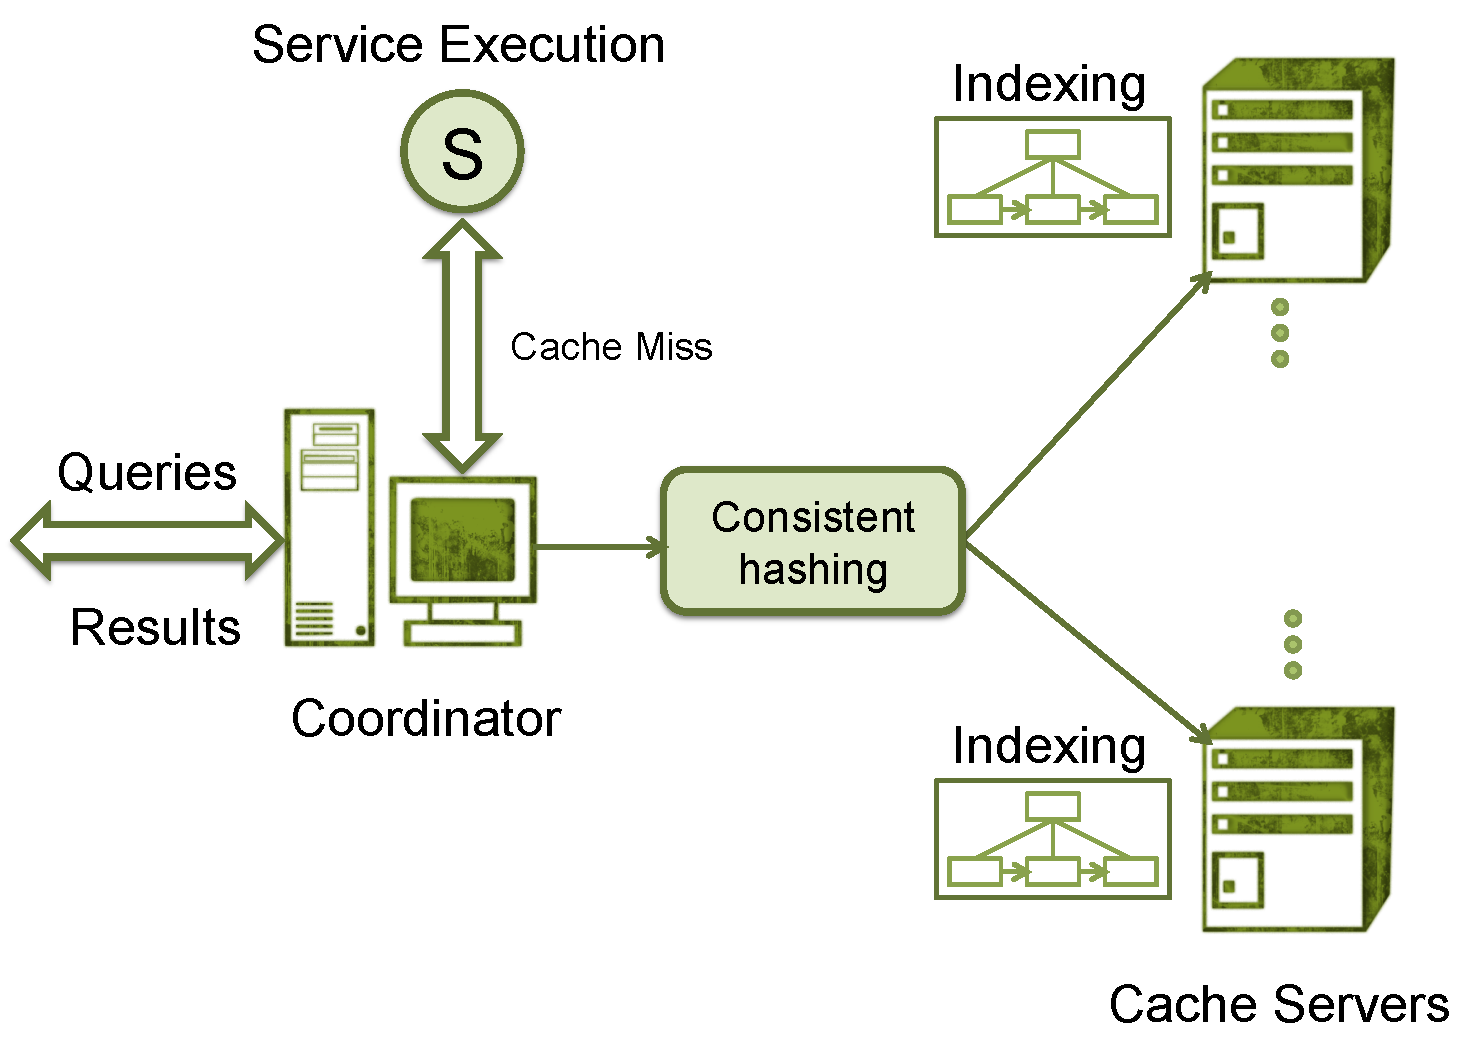
\includegraphics[scale=0.5]{figures/arch.pdf}
\end{center}
\caption{Client-Server Architecture of the Elastic Cache}
\label{fig:architecture}
\end{figure}

Our system is composed from a number of Cloud nodes including a
\emph{Coordinator node} and a set of independent \emph{Cache nodes} indexed by
consistent hashing as seen in Figure~\ref{fig:architecture}. The coordinator is
in charge of several different roles:
\begin{itemize}
	\item Interfacing with the users through a simple key-value API.
	\item Determining which cache node might contain the data and routing the
		query to it.
	\item Monitoring the capacity of nodes and determining when to allocate a new
		node and overflow into it.
	\item Retrieving, returning, and caching data in the event of a cache miss.
\end{itemize}
% section Elastic_Key-Value_Cache_System (end)

\section{Cache Coordinator} % (fold)
\label{sec:Cache_Coordinator}
% Request handling
Users interact directly with the coordinator, performing queries in a simple
and straightforward manner. Within our system, this is done as a simple
key-value API, however more complex APIs are conceivable for different domains.
When receiving a request, the coordinator then maps the query to one of the
cache nodes it manages and proceeds to redirect the query there. In the event
of a cache hit, the coordinator receives the data and redirects it to the user.
On a miss, the coordinator is then in charge of retrieving the data that the
user requested. Depending on the domain of application, this can entail
different things. For example, the coordinator could be expected to go and
fetch a web page from the primary server, or it may be expected to schedule and
invoke a service application. Once the results have been retrieved, the
coordinator then sends the data to the user and places it within the cache.

% Consistent hashing mechanism
One of the initial challenges of the cache was in identifying precisely which
cache node would contain the key-value pair that the user is interested in.
While one might expect that a simple hashing mechanism would provide precisely
the utility necessary, the elastic nature of the system prevents that. As nodes
are added to and removed from the system, a very large number of the key-value
pairs would need to be rehashed to accommodate. This obviously becomes
prohibitive the larger the cache becomes as there would then be a greater
number of key-value pairs being moved about, necessitating a tremendous amount
of network activity between the cache nodes (as they migrate data into one
another).

\begin{figure}
\begin{center}
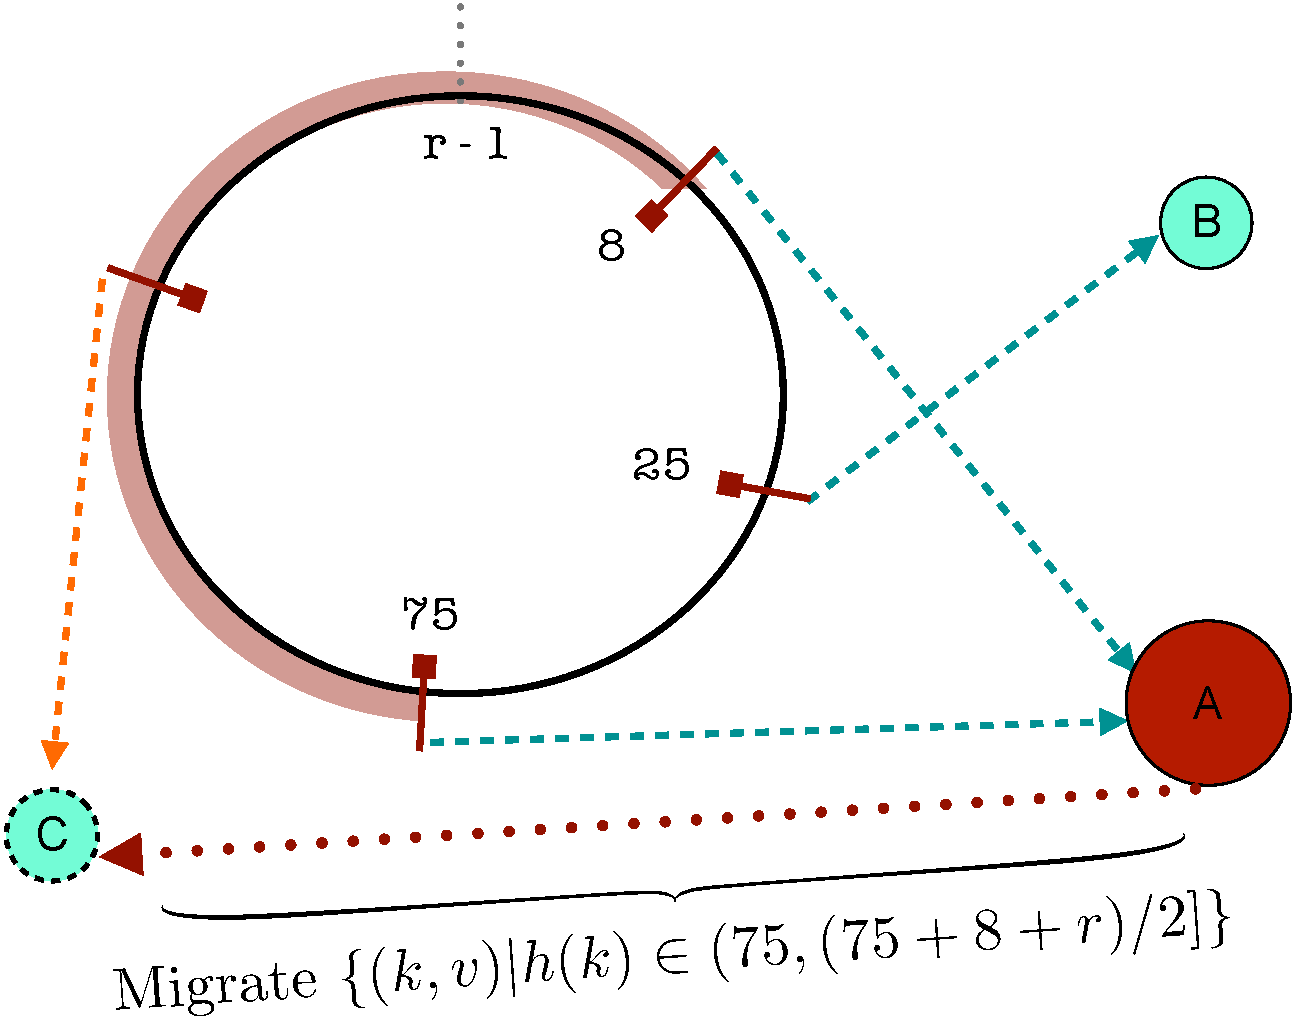
\includegraphics[scale=0.5]{figures/hashing.pdf}
\end{center}
\caption{Consistent Hashing}
\label{fig:hashing}
\end{figure}

Instead, we implement consistent hashing (CITE - Karger 1997), a mechanism well
adapted to the highly dynamic nature of our problem. In fact, consistent
hashing is used within the even more-volatile systems of Peer-to-Peer
transfers. The circular hash ring that hash buckets are stored in allow for
easy splitting and rehashing of each node. Each node being determined by the
clockwise-successor of $key mod r$ means that the hash does not need to be
reconstructed from scratch each and every added node.

As an example, consider Figure~\ref{fig:hashing}, which depicts a consistent
hashing system composed of two nodes, $A$ and $B$. The circular hash range
rotates between $0$ and $r-1$, and consists of several buckets placed randomly
or strategically along the ring. Each bucket stores a pointer to a physical
storage node. An additional static hash function then maps key-value pairs
$(k,v)$ onto the hash ring. For example, a function that determines the
clockwise-successor for some $k \textrm{mod} r$ would begin by hashing to some
value on the hash ring and then finding the nearest succeeding bucket in
clockwise fashion. To continue the example in the figure: a $(k,v)$ pair
hashing onto 35 would follow the ring to node $A$ as referenced by bucket 75.

% Load balancing
In addition to interfacing with the user, the coordinator is responsible for
monitoring the capacity and status of the cache. As need arises, either through
demand or overflow, the coordinator takes control of splitting full nodes by
allocating new ones and migrating portions of the data from one to the other.

Figure~\ref{fig:hashing} additionally shows that node $A$ is overflown and a
new node, $C$, has been allocated from the cloud to be incorporated into our
system. Assuming that the range between $(75,8]$ on the hash ring is crowded
with too many keys hashing onto $A$, we can place $C$ strategically, such that
a large number of the keys in $(75,8]$ will be hashed into it, alleviating the
load on $A$. For example, the bucket could be placed at $(75 + 8 + r)/2$ and
the $(k,v)$ pairs hashing into $(75, (75 + 8 + r)/2]$ are migrated into node $C$.

In addition to simply splitting and migrating, the coordinator is also where we
identified areas for future improvement (CITE - IJNGC2011). From this
macro-level control area, we proposed a more intelligent mechanism for
controlling the overall cache hierarchy. Though this area was developed in
parallel with the work of this paper and falls outside of its scope, we offer a
high level overview of these mechanisms.

At the macro level, the cache coordinator is concerned with managing the size
of each tier in the hierarchy and its associated costs. Users have the option
to input any of the following:
\begin{inparaenum}[(1)]
  \item a cost constraint parameter $C$,
  \item a cost-priority parameter $P_c, (0 < P_c < 1)$ and
  \item a list of Cloud resource usage costs.
\end{inparaenum}
The objective of the coordinator is then to maximize cache performance given
these constratings. The cost-priority parameter allows users to configure the
importance of performance against cost. Additionally, the macro level is
responsible for planning the capacity and using an Artificial Neural Network
(ANN), intelligently predicts the underlying cache nodes' memory and disk loads
at any time in the future. Time series forecasting is then used to model future
events and allows for the coordinator to plan and accomodate accordingly.

% section Cache Coordinator (end)

\section{Cache Node} % (fold)
\label{sec:Cache_Node}
% Data storage

\subsection{Indexing}
\label{sub:cache_indexing}
Each cache node is, at its most basic level, responsible for only a few tasks.
Intuitively, as this is the area where the key-value pairs are actually stored,
each node must implement functionality that allows for \emph{insertion} and
\emph{retrieval} at the least. We extend this to include functionality for
\emph{inserting}, \emph{deleting}, \emph{searching}, \emph{evicting}, and
\emph{migrating} data. At its inception, and in order to facilitate fast
searches and retrievals, each participating node used only its memory for
storage and employs an application-specific \emph{indexing scheme}. This choice
of indexing scheme impacts both the split and migration time of each node, as
support for fast range queries allows the system to quickly determine which
records need to be transferred. Furthermore, the performance of the entire
cache is dependent upon the speed of record retrieval and the speed at which it
can determine hits and misses.

In previous works\cite{chiu_ccgrid11,chiu_ijngc11}, we have analyzed three
different indexing schemes: \bptrees, Extendible Hashing, and Bloom filters. We
concluded that \bptrees scale well regardless of system parameters, and
Extendible Hashing, with its constant-time exact-match searches, could
outperform \bptrees if their parameters are chosen appropriately. However, if
the cache system is volatile and migration is invoked often, Extendible Hashing
indexing schemes will result in increasingly poor migration performance. We
also note that Counting Bloom Filters should generally be avoided as an
indexing scheme for elastic key-value storage. As a caveat, however, CBF may
scale well for applications relying on space-efficient structures. We also make
note of the interesting observation that CBF migration overheads become better
over time. As a result of this, we chose to employ \bptrees for our purposes
and detail their operation here.

\subsubsection{\bptrees} % (fold)
\label{subsub:b_trees}
B-Trees and \bptrees are used in many of today's systems. The \bptree is a
multilevel indexing scheme that automatically adjusts the number of levels
depending upon the file size and stores all of its records in the leaf nodes.
Each record is stored in ascending order from left to right and each leaf node
is linked to the next and previous nodes. In this way, its design is
specifically crafted to accelerate queries over a range of
values\cite{navathe,ullman}. In terms of retrieval, \bptrees are balanced data
structures, where all paths from the root to any leaf have the same length
(similar to binary trees, with approximately log$_2 n$ depth).

\begin{figure}
\begin{center}
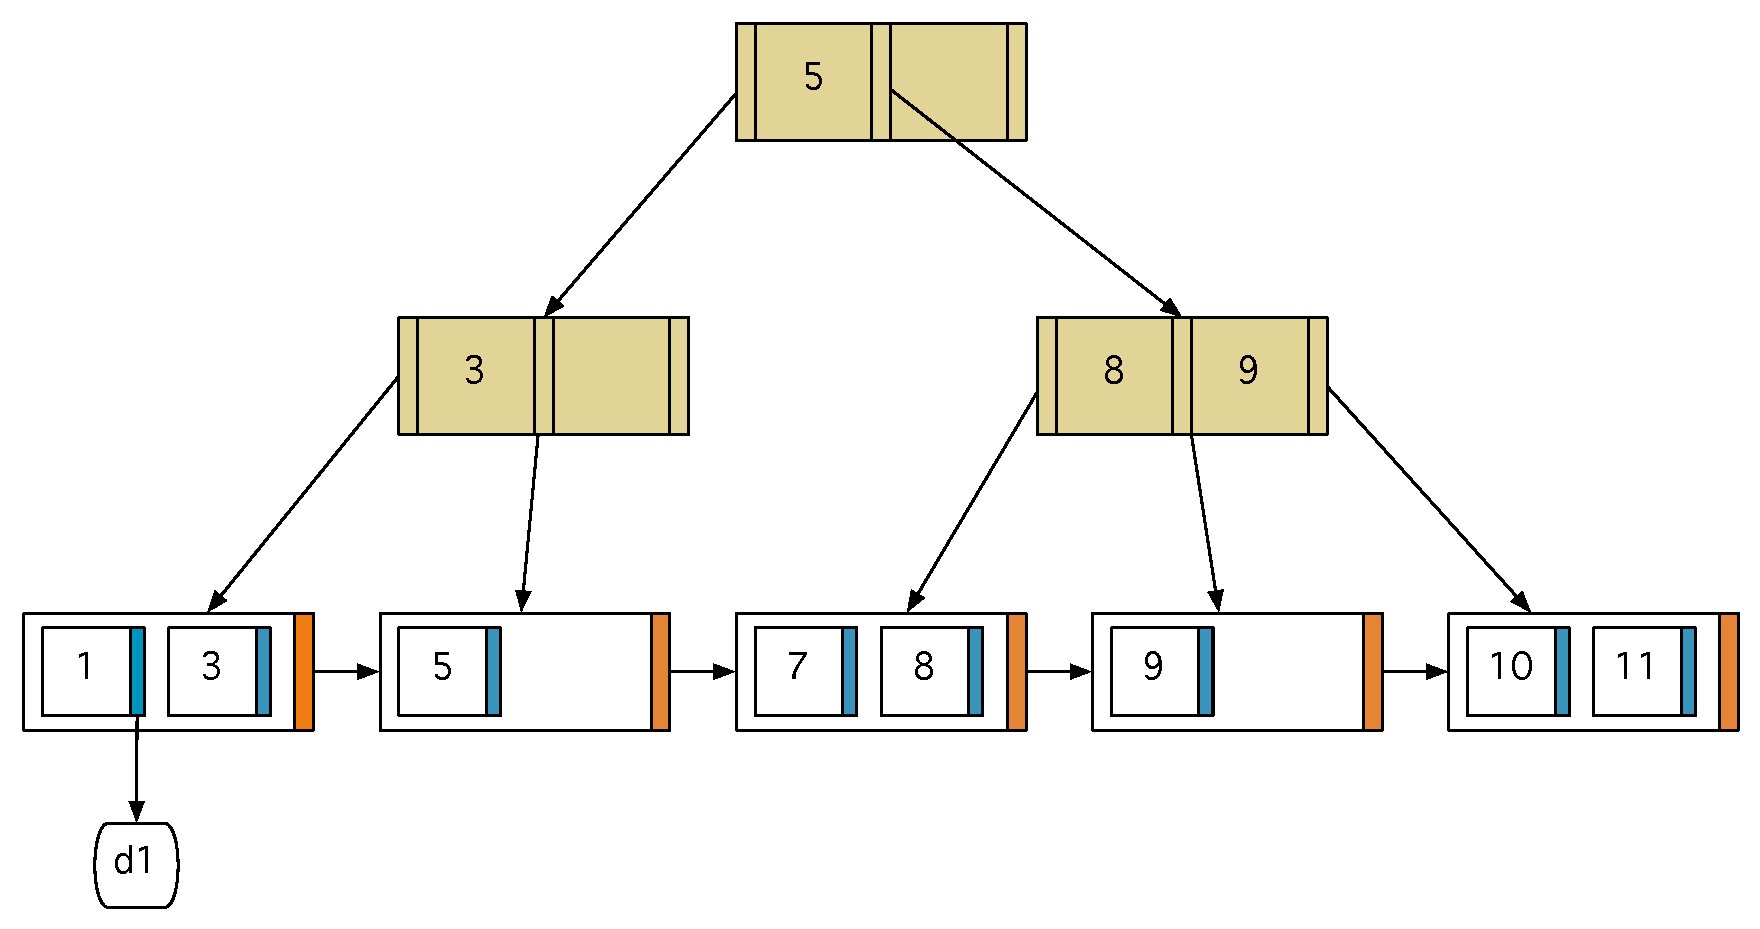
\includegraphics[scale=0.5]{figures/bplustree.pdf}
\end{center}
\caption{\bptree structure}
\label{fig:bplustree}
\end{figure}

Structurally, \bptrees are composed as shown in Figure~\ref{fig:bplustree}.
Internal nodes, those colored beige, act as pointers to other nodes in the
structure. All keys in the left branch of the key \emph{K} are less than or
equal to \emph{K}, while all keys to the right are greater than \emph{K}. While
searching, we compare the search key with the entries in the tree until such a
point as we reach the leaf node. Leaf nodes, those colored white, contain the
stored keys and pointers to the physical data location (blue). Additionally, in
order to assist with range queries, leaf nodes also contain a pointer to the
next leaf node, in order (orange).

With this sort of structure, we can see that range queries are made quite
simple and quick. Given a range $[k_{start}, k_{end}]$ we begin by searching to
find $k_{start}$ then proceed to iterate through the leaves until we find a
node greater than $k_{end}$. The search then returns the set of data identified
in that range. Due to this support, we expect the \bptree integration to be
well suited to elastic cache. Quick access to ranges of data should lead to
much faster data migration in the event of node additions. Data migration,
which is composed of a set of key deletions, can again be efficiently managed
in the same way as a range query is. The \bptree migration algorithm is shown
in Algorithm~\ref{alg:migrate1}.

\begin{algorithm}[htp]
\small
\caption{\label{alg:migrate1}BT\_Migrate($k_{start}$, $k_{end}$)} \begin{algorithmic}[1]
\STATE $\triangleright$ manipulate B$^+$-tree index and transfer the keys in form of a string, $keys$
\STATE $end \leftarrow false$
\STATE $\triangleright$ $L =$ leaf initially containing $k_{start}$ 
\STATE $L \leftarrow btree$.search($k_{start}$)
\WHILE{$(\neg end \wedge L \neq NULL)$}
 \STATE $\triangleright$ each leaf node contains multiple keys
 \FORALL {$(k,v) \in L$}
   \IF {$k \le k_{end}$}
     \STATE $keys$.append($k$, $v$)
     \STATE $btree$.delete($k$)
   \ELSE
     \STATE $end \leftarrow true$
     \STATE break
   \ENDIF
 \ENDFOR
 \STATE $L \leftarrow L$.next()
\ENDWHILE
\STATE return $keys$
\end{algorithmic}
\end{algorithm}

% subsubsection bplustree (end)

% subsection Indexing (end)

\subsection{Eviction} % (fold)
\label{sub:cache_eviction}

As mentioned, each cache node is also given the ability to evict data. As the
node becomes nearer to full, if the coordinator has not decided to split it
and migrate data out, it must be able to make room for additional data. As with
\emph{indexing strategies}, \emph{eviction strategies} are also
application-specific. Choices in eviction strategy are reflected in the hit-
and miss-rates of the cache, which further dictate the overall performance of
the system. As hinted at by Figure~\ref{fig:architecture}, cache misses lead to
the execution of, often computationally and time-expensive, services. In
Chapter~\ref{chap:Eviction_Strategies}, we present background information on two
common indexing structures: First-In First-Out (FIFO), Least Recently Used
(LRU), in addition to a scoring-based algorithm of our own creation.

% subsection cache_eviction (end)

\subsection{Migration} % (fold)
\label{sub:cache_migration}

Finally, each cache node is individually responsible for handling the migration
of data from one instance to the next. Given that the indexing scheme can be
determined on a per-node basis (e.g.\ one node uses a B$^+$-tree while the
other uses Extendible Hashing), implementation of the migration command is
similarly determined. For example, in Figure~\ref{fig:hashing}, where keys are
being migrated from $A$ to $C$, the coordinator would inform cache node $A$ to
migrate keys in the range $(75,(75 + 8 + r)/2]$ to node $C$. Node $A$ would
then connect directly to node $C$ and begin its migration. As mentioned, this
has implications on the selection of the \emph{indexing strategy}. With
migrations occurring over a range of keys, being able to swiftly do searches
over that range becomes very important.

% subsection cache_migration (end)

% section Cache_Node (end)

\section{Amazon AWS} % (fold)
\label{sec:Amazon_AWS}
Amazon's Web Services (AWS) are composed of a wide range of tools for cloud
computing. For the purposes of our cache, we make heavy usage of the Elastic
Compute Cloud (EC2) service. Within EC2, nodes (\emph{instances}) are virtual
machines that can launch snapshots (\emph{images}) of various system
configurations. These snapshots can be loaded onto a number of different
\emph{instance types} of varying capabilities and costs.

For example, a small EC2 instance ({\tt m1.small}) according to
AWS\cite{amazonEC2InstanceTypes} at the time of writing, contains $1.7$ GB of
memory, $1$ virtual core with $1$ EC2 Compute Unit\footnote{``One EC2 Compute
  Unit provides the equivalent CPU capacity of a 1.0-1.2 GHz 2007 Opteron or
2007 Xeon processor. This is also the equivalent to an early-2006 1.7 GHz Xeon
processor[\ldots]'', http://aws.amazon.com/ec2/instance-types/}, $160$ GB of
disk space and can be run on a $32$-bit \emph{or} $64$-bit platform. AWS
further defines that a small instance has \emph{moderate} network I/O. Though
the exact definition of \emph{moderate} is not defined by AWS, they do make the
following claim\cite{amazonEC2InstanceTypes}:

\begin{quote}
  The different instance types will provide higher or lower minimum performance
  from the shared resources depending on their size. Each of the instance types
  has an I/O performance indicator (\emph{low}, \emph{moderate}, or
  \emph{high}). Instance types with \emph{high} I/O performance have a larger
  allocation of shared resources.  Allocating larger share of shared resources
  also reduces the variance of I/O performance. For many applications,
  \emph{low} or \emph{moderate} I/O performance is more than enough. However,
  for those applications requiring greater or more consistent I/O performance,
  you may want to consider instances with \emph{high} I/O performance.
\end{quote}

Another instance type we look at, the Extra Large Instance ({\tt m1.xlarge}),
consists of $15$ GB of memory, $4$ virtual cores with $2$ EC2 Compute Units
each, $1,690$ GB of disk space, \emph{high} I/O performance, and can only be
run on a $64$-bit platform. The costs (USD) of running these compute instances
in the US East (Virginia) region are outlined in
Table~\ref{tab:costs_ec2_instance}. The costs of data transfer in and out of
instances are outlined in Table~\ref{tab:costs_ec2_transfer}.

\begin{table}[htp]
  \begin{center}
    \begin{tabular}{|l|l l|}
      \hline
      \multicolumn{1}{|c}{\textbf{Instance Type}} &
      \multicolumn{1}{|c}{\textbf{Linux/UNIX Usage}} & 
      \multicolumn{1}{c|}{\textbf{Windows Usage}}\\
      \hline
          Small (Default) & \$0.080 per Hour & \$0.115 per Hour\\
                   Medium & \$0.160 per Hour & \$0.230 per Hour\\
                    Large & \$0.320 per Hour & \$0.460 per Hour\\
              Extra Large & \$0.640 per Hour & \$0.920 per Hour\\
      \hline
    \end{tabular}
    \caption{EC2 Standard On-Demand Instance Cost}
    \label{tab:costs_ec2_instance}
  \end{center}
\end{table}

\begin{table}[htp]
  \begin{center}
    \begin{tabular}{|l | c|}
      \hline
      \multicolumn{1}{|c}{} & \textbf{Pricing} \\
      \multicolumn{2}{|l|}{\textbf{Data Transfer IN}} \\
      \hline
      All data transfer in & \$0.000 per GB \\
      \hline
      \multicolumn{2}{|l|}{\textbf{Data Transfer OUT}} \\
      \hline
             First 1 GB / month & \$0.000 per GB\\
            Up to 10 TB / month & \$0.120 per GB\\
             Next 40 TB / month & \$0.090 per GB\\
      \hline
    \end{tabular}
    \caption{EC2 Internet Data Transfer}
    \label{tab:costs_ec2_transfer}
  \end{center}
\end{table}

\begin{table}[htp]
  \begin{center}
    \begin{tabular}{|l | l|}
      \hline
      \textbf{Medium} & \multicolumn{1}{c|}{\textbf{Cost}} \\
      \hline
      S3 & \$0.125 per GB-month of provisioned storage\\
         & \$0.01 per $1,000$ in-requests\\
         & \$0.01 per $10,000$ out-requests\\
      \hline
     EBS & \$0.10 per GB-month of provisioned storage\\
         & \$0.10 per 1 million I/O requests\\
      \hline
    \end{tabular}
  \end{center}
  \caption{Persistent Storage Costs}
  \label{tab:costs_persistent}
\end{table}

Amazon also provides two frameworks for persistent storage. The most popular of
them, the Simple Storage Service (S3), provides a key-value store with a simple
FTP-style API: {\tt put}, {\tt get}, and {\tt del}. The unique keys are
represented by a filename with the actual value of each data object being the
file itself. Though objects are limited to a maximum of $5$ GB in size, the
total number of objects that can be stored in S3 is unlimited. The S3
architecture has also been designed to be both highly reliable and available.

The second option, Elastic Block Storage (EBS) works in tandem with EC2
instances. The EBS service provides a persistent disk space that can be mounted
from within a running EC2 instance. Though the size of an individual EBS volume
is limited to $1$ TB and can only be attached to a single instance at a time,
any instance can mount multiple EBS volumes. From within the EC2 instance, the
mounted EBS volume can then be treated a part of the local filesystem.
Table~\ref{tab:costs_persistent} shows the costs of these two persistent
storage frameworks.

\subsection{Tradeoffs} % (fold)
\label{sub:aws_tradeoffs}
There are a number of tradeoffs involved in deploying our cache over the AWS
resources. Here we discuss these tradeoffs briefly.

\subsubsection{In-Instance-Core Option} % (fold)
\label{subsub:in_instance_core}
By supporting our cache over EC2 nodes, we can harness several advantages in
terms of flexibility and throughput. Depending on our purposes, it may be
possible and desirable to store all cached data directly in memory, reducing
access time. Because small instances consist of only 1.7 GB of memory, we may
need to allocate more instances to cooperate in establishing larger capacity.
We could also serve the same purpose by allocating an extra large instance with
15 GB of memory. The instance could, however, overfit our cache requirements,
betraying cost-effectiveness. For this reason, we expect that a memory-based
cache would be the most expensive, while affording the highest performance.
% subsubsection in_instance_core (end)

\subsubsection{In-Instance-Disk Option} % (fold)
\label{subsub:in_instance_disk}
When larger quantities of data are expected in the cache, we can also store
data on the instance's disk. Even the small EC2 instances provide significant
amounts of disk space (160 GB), which dramatically increases our overall
capacity beyond that of a memory-based cache. With almost 100 times more
storage capacity on the disk than in RAM, this means a tremendous reduction in
the number of instances we need to allocate purely for capacity reasons.
However, this extra capacity comes at a cost: disk accesses can be very slow
compared to the in-memory cache if request rates are high. That said, if the
average data size is large, disk access overheads may be amortized over time.
We expect that the disk-based solution should be cheaper than the memory-based
solution, with slightly lower performance benchmarks depending on the average
data size.
% subsubsection in_instance_disk (end)

\subsubsection{Persistent Options} % (fold)
\label{subsub:persistent_options}
In both the memory-based and disk-based solutions, there is no accounting for
data persistence. Put simply: if a node fails, is shut down, or is otherwise
removed from the cache, any data stored on it is considered to be lost. Even if
the data is stored on ``disk,'' when the Cloud provider reclaims the resources
for that cache node, the data stored within is wiped clean so that the resource
may be used again. In addition to recovering from node failure, it can be
beneficial to stop and restart cache nodes during peak/non-peak times as a
mechanism for saving usage costs, and so we introduce a third tradeoff option
that allows for persistence.

The most simple persistence method is to directly utilize S3 to store cached
data. This is convenient for the application developer as we eliminate the
need for additional indexing logic, using S3's simple API instead, in addition
to being very inexpensive. Additionally, because S3 is independent from
Amazon's EC2 system, we can store data without having to allocation additional
instances for storage. Due to the reliability and availability guarantees of
S3, however, the storage architecture is provided in such a robust fashion,
with support for replication and consistency, that it will likely impact
performance. In addition, data transfer costs are equivalent to those of EC2
instances, and so despite the low storage costs, in high-throughput
environments, we can expect that S3 will not provide significant cost benefits.

Additionally, as we alluded to previously, the Elastic Block Storage (EBS)
system provides another means of data persistence. One primary difference
between S3 and EBS is that EBS volumes are inherently less accessible. In
contrast to S3, EBS volumes do not provide unlimited storage, and thus their
size must be predefined by users before being mounted onto an EC2 instance.
However, because these volumes are mounted to the instance, this suggessts the
potential for higher throughput than S3, where communications occur through
high-level SOAP/REST protocols transmitted over HTTP.\ From a cost analysis
standpoint, EBS invokes additional storage and request overhead to the
hourly-based EC2 instance costs.
% subsubsection persistent_options (end)

% subsection aws_tradeoffs (end)

% section Amazon_AWS (end)
